\chapter{Metodi e Strumenti per l'Innovazione}

Introduciamo ora una serie di metodi di lavoro e strumenti nati per facilitare la progettazione e realizzazione di prodotti e sistemi innovativi. 

\begin{flushleft}
\textit{ \textbf{Innovazióne} s. f. [dal lat. tardo innovatio -onis]. L’atto, l’opera di innovare, cioè di introdurre nuovi sistemi, nuovi ordinamenti, nuovi metodi di produzione. In senso concreto, ogni novità, mutamento, trasformazione che modifichi radicalmente o provochi comunque un efficace svecchiamento in un ordinamento politico o sociale, in un metodo di produzione, in una tecnica, ecc. [Treccani]}
\end{flushleft}

In innovazione, l'applicazione della filosofia HCD diventa di vitale importanza dal momento che un prodotto o servizio per essere innovativo deve essere prima di tutto apprezzato dagli utenti e quindi utilizzato.

\textbf{Cosa vuol dire innovare? Esiste un solo modo di fare innovazione?}

\section{Disruptive Innovation}
\begin{flushleft}
	\textit{\textbf{People don’t want to buy a quarter-inch drill. They want a quarter-inch hole!} - Professor Theodore Levitt, Harvard Business School}\\

\end{flushleft}

La maggior parte dell'innovazione è fatta come miglioramento incrementale di prodotti o sistemi già esistenti. I nuovi condizionatori d'aria, per esempio, hanno motori e gas più efficienti rispetto al passato ma il loro funzionamento è basato sul principio della macchina frigorifera che fu proposto per la prima volta nel 1835.
Questo approccio all'innovazione fatta attraverso piccole migliorie apportate ad un sistema stabile è il più comune. Questo processo passo-passo è molto affidabile, consente di raggiungere buoni risultati con investimenti tutto sommato contenuti e di mantenere invariata la struttura delle aziende (produttori) e della società (consumatore). Questo processo di innovazione incrementale ha però bassissime probabilità di portare ad una modifica sostanziale del prodotto/processo su cui è applicato.

L' \textbf{Innovazione Incrementale} punta infatti al mantenimento della competitività aziendale tramite un processo passo-passo dove si fa un aggiornamento alla volta. Nel paradigma di innovazione incrementale la clientela di riferimento è stabile e definita e non si punta solitamente ad espandere il business verso altre nicchie di clientela.

In generale però, quando si parla di innovazione, ci si aspetta di trovarsi davanti ad un prodotto o servizio che cambi radicalmente il modo in cui si fanno le cose. Qualcosa di nuovo, destinato a "cambire il mondo". Questo tipo di innovazione è detto \textbf{disruptive innovation} e si basa su una forte discontinuità con il passato. L'innovazione di tipo dirompente è spesso alla base dei modelli di business e di sviluppo delle startup ed è uno degli elementi di differenziazione che c'è fra una startup e un'impresa tradizionale.

Il termine Disruptive Innovation è stato utilizzato per la prima volta da Clayton Christensen nel libro ``Il dilemma dell’innovatore'' del 1997 per spiegare come i processi innovativi attuati dalle aziende seguano principalmente due paradigmi.

Nella \textbf{Disruptive Innovation}, si punta quindi a conquistare quelle nicchie di clientela che risultano ancora irraggiungibili tramite i prodotti, le tecnologie e i sistemi esistenti. Per fare questo si mette in discussione l'intero impianto tecnologico e di business del prodotto e si ridisegna il tutto sulla base delle moderne tecnologie così da cercare di acquisire nuovi mercati inesplorati e quindi più fertili.

E' sempre molto difficile definire a posteriori quale prodotto o tecnologia è/sia stato disruptive e quale no. I prodotti, i sistemi e le tecnologie diventano ovvie un secondo dopo che sono state accettate dal mercato e quindi ci si dimentica velocemente di come questi abbiano cambiato il mondo in cui viviamo. 

Si ha innovazione dirompente quando un prodotto è in grado di offrire performance e possibilità di utilizzo completamente impensabili rispetto alle precedenti soluzioni o di definire un mercato di riferimento completamente nuovo.

Un indiscutibile esempio di innovazione dirompente è sicuramente stato \textbf{Internet}. Grazie alla Rete sono nati sistemi di comunicazione, modelli di business, prodotti e culture che prima non esistevano. Internet ha cambiato il mondo in una maniera così radicale da non consentire un ritorno al passato. E' indubbio che oggi sarebbe impossibile vivere senza rete.

Il settore dove invece regna sovrana l'innovazione incrementale è sicuramente quello dell'automotive. Ogni anno escono auto che consumano un pochino meno, che sono un pochino più spaziose, comode e preformanti dei modelli precedenti ma la tecnologia che sottostà questo processo è sempre la stessa. Il primo brevetto di un motore a combustione interna è del 1853 e da allora i suoi principi di funzionamento non sono mai stati modificati radicalmente ma solo ottimizzati ed evoluti.
Ma la disruptive innovation sta arrivando anche nel settore dell'automotive e nel giro di pochi anni le auto a guida autonoma e le motorizzazione elettriche diventeranno ovvie e il mondo dei trasporti non sarà più quello di una volta. Ci troveremo da un giorno all'altro a considerare ciò che ieri era fantascienza una nuova ovvia normalità e a considerare ciò che ieri era la norma preistoria.

a questo link (\url{http://www.concept.by/approfondimenti/innovazione-radicale/}) potete trovare un'interessante sintesi del libro "il dilemma dell'innovatore" in cui per spiegare il concetto di innovazione dirompente è  riportata la storia degli hard disk da 3,5 pollici.

La disruptive innovation è quindi il campo di gioco delle startup e di tutti quegli innovatori che lavorano per proporre nuovi modelli di business innovativi capaci di scalare rapidamente e globalmente. Non è un caso che aziende di successo, un tempo startup, come Airbnb, Amazon, Google, Facebook e Tesla tra le più recenti, ma anche le più longeve come Apple e Microsoft abbiano profondamente innovato i propri mercati in modo dirompente ed oggi rappresentino per tutti il concetto di innovazione. 

\begin{figure}[!h]
	\centering
	\includegraphics[width=\textwidth]{"immagini/Disruptive Innovation"}
		\caption{Sustaining e Disruptive innovation a confronto. Fonte: https://hcldr.wordpress.com/2017/01/10/disruptive-innovation-in-healthcare/}
\end{figure}

\textbf{Non si può fare innovazione dirompente senza una forme di pensiero e progettazione antropocentrica.}\\

Che vogliate cambiare il mondo dei trasporti (Uber, Tesla), andare su Marte (SpaceX), cambiare il modo in cui si sviluppano i servizi web (AWS, Microsoft Azure) o cambiare il modo in cui si va in vacanza (AirBnB, Booking) prima o poi il vostro prodotto o servizio avrà un utente, un acquirente, un finanziatore e un fan. Se non vi curerete di loro fin dalle prime fasi di progettazione la vostra sarà un'azione dirompente solo per voi stessi (e per il vostro portafoglio) perchè un prodotto o servizio che nessuno utilizza non fa innovazione.

\section{Human Centered Design Process}
IDEO, una delle più grandi agenzie di design al mondo ha deciso di adottare lo Human Centerd Design in ogni suo progetto. IDEO ha inoltre creato intorno ai principi dello HCD una serie di strumenti di sviluppo e design che sono diventati molto popolari nel mondo del design di prodotto.

In particolare, IDEO ha proposto un vero e proprio metodo di progettazione basato sui fondamenti dell'HCD lo Human Centered Design Process.

Se lo Human Centered Design pone l'accento sul fattore umano, lo Human Centered Design Process considera l'attività umana come un ombrello al di sotto del quale interagiscono i fattori umani, tecnologici e sociali.
Pertanto, rispetto ad un processo "tradizionale", lo Human Centered Design Process può essere definito come: \textit{"Un processo ispirato da comportamenti piuttosto che dalle statistiche, che si svolge in un contesto naturale piuttosto che in un ambiente controllato, e si basa su conversazioni aperte piuttosto che su interviste trascritte"}

Tutto questo processo, che potrebbe apparire astratto, in realtà poggia su un solido e preciso percorso di progettazione diviso in 3 fasi: Ispirazione, Ideazione e Implementazione.

\textbf{L'ispirazione}, la scoperta, sono legate all'osservazione dell'utente e dei suoi bisogni. Per IDEO, ad esempio, si tratta di capire come migliorare uno strumento osservando il modo in cui la persona utilizza quello strumento.  Quindi il risultato che ne verrà fuori sarà un design legato alla realtà dei fatti e delle situazioni e non alle ipotesi dei progettisti.

\textbf{L'ideazione} si basa sui contenuti appresi durante la fase dell'osservazione. Questi vengono messi in discussione e affrontati in gruppo, un'interazione da più ambiti in cui l'obiettivo è quello di ragionare su più idee possibili rimanendo focalizzati sui bisogni e le necessità dei destinatari. Da concetti ideali, come quelli della prima fase, si cerca di interpretare le conoscenze assunte per arrivare a qualcosa di più tangibile, magari tramite la creazione di un semplice prototipo. 

Il prototipo non deve essere definitivo né perfetto o completo di tutte le funzionalità necessarie. Serve come punto di partenza per un confronto con i destinatari del progetto. Non è un primo, vago tentativo di soluzione, ma fa sì che le risposte future risponderanno alle esigenze del target.

Incamerato il feedback, sarà più semplice continuare a testare e confrontarsi per arrivare all'attesa soluzione, senza inciampare lungo il cammino per arrivare alla fase di \textbf{implementazione}.

Ciascuna di queste fasi viene svolta dal team con una approccio a fisarmonica. All'inizio si lavora per produrre idee e soluzioni in quantità (divergenza), ci si focalizza poi nella selezione, fusione e integrazione delle proposte così da distillare i risultati e produrre un numero ridotto di soluzioni (convergenza) da passare alla fase successiva.

VIDEO di presentazione dello HCD process di IDEO \url{https://vimeo.com/106505300}.

\begin{figure}[!h]
	\centering
	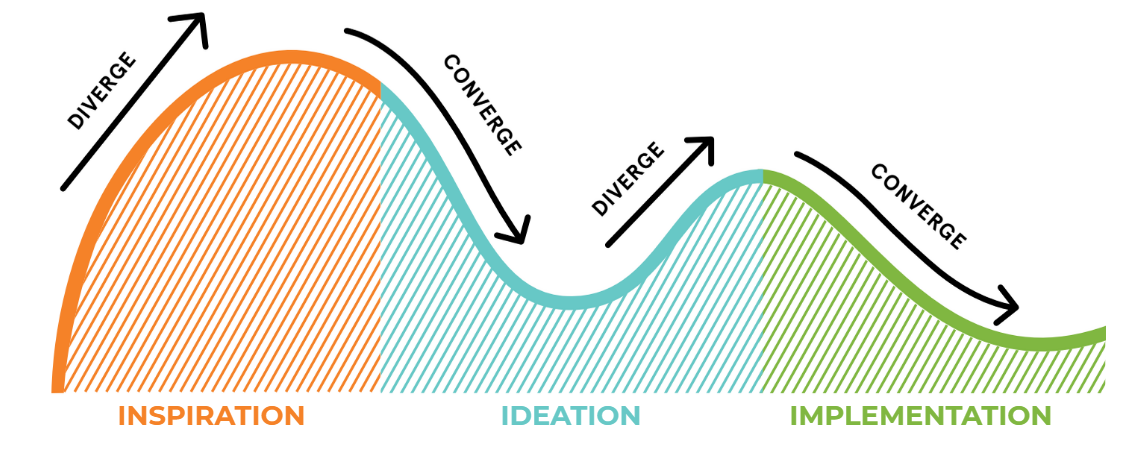
\includegraphics[width=0.8\textwidth]{immagini/HCD-process.png}
	\caption{HCD process. é un processo diviso in 3 fasi dove è sempre applicato un metodo di lavoro a fisarmonica che prevede una fase di divergenza e una di convergenza. Fonte https://blog.movingworlds.org/human-centered-design-vs-design-thinking-how-theyre-different-and-how-to-use-them-together-to-create-lasting-change/} 
	\label{hcd-process}
\end{figure}

\section{Design Thinking}
Il Design Thinking È un approccio all’innovazione che poggia le sue fondamenta sulla capacità di risolvere problemi complessi utilizzando una visione e una gestione del progetto basata sulla creatività. 

Tale approccio è stato codificato attorno agli anni 2000 in California dall’Università di Stanford. È centrato sulle persone (antropocentrico) e si basa sull’abilità di integrare capacità analitiche con attitudini creative. In genere viene applicato da un team multidisciplinare che ha come obiettivo quello di trovare una soluzione innovativa ad un problema (disruptive) tenendo conto del gradimento (Human-centered) di essa, della redditività indotta e della sostenibilità economica (business).

In origine, il Design Thinking nacque come approccio all’innovazione adottato da agenzie e studi di design. Oggi invece, la sua diffusione sta permeando in settori molto diversi, anche in quelli ritenuti più distanti, fino a qualche anno fa. Il design thinking sta diventando infatti uno dei metodi di riferimento utilizzati dalle startup e da aziende innovative per la realizzazione di prodotti tecnologici, per la trasformazione digitale e la progettazione di software e interfacce.

Il DT ha 3 obbiettivi fondamentali:

\begin{enumerate}
    \item avvicinarsi al cliente;
    \item favorire la creatività e generare idee;
    \item sperimentare rapidamente le idee attraverso la realizzazione di prototipi.
\end{enumerate}

Tuttavia ridurre il DT all’elenco degli obbiettivi, dei settori di utilizzo o dei tool che lo caratterizzano è estremamente limitante. E' invece molto più efficace ed importante comprendere il mindset e la prospettiva che caratterizzano i processi di DT. Questo perchè, quotidianamente vengono proposti nuovi metodi, strumenti e tecnologie a supporto di questa modalità di progettazione e pertanto andare a trattarla sulla base degli strumenti più utilizzati è scorretto e limitante.

Relativamente all'approccio DT, Roberto Verganti Professore di Leadership and Innovation alla Stockholm School of Economics afferma: \textit{Si tratta di ribaltare il classico triangolo, tipico delle business school, che pone nel vertice in alto il business e alla base people e technology, a indicare come l’obiettivo dell’impresa sia l’uso dell’innovazione per creare business value a favore degli stakeholder, grazie a prodotti che soddisfino i bisogni delle persone attraverso l’uso delle tecnologie.} figura \ref{fig:dt_piramide}.

\textbf{L’approccio Design Thinking pone nel vertice in alto le persone.}\\

\textit{Partiamo dai sogni e dai problemi delle persone e creiamo prodotti che li soddisfino. Se ci riusciremo lo sviluppo del business ne sarà la naturale conseguenza.} 

In un processo di sviluppo basato su design thinking il business e la tecnologia sono solo degli strumenti per raggiungere l'obbiettivo primo, la soddisfazione dell'utente.

\begin{figure}[!h]
	\centering
	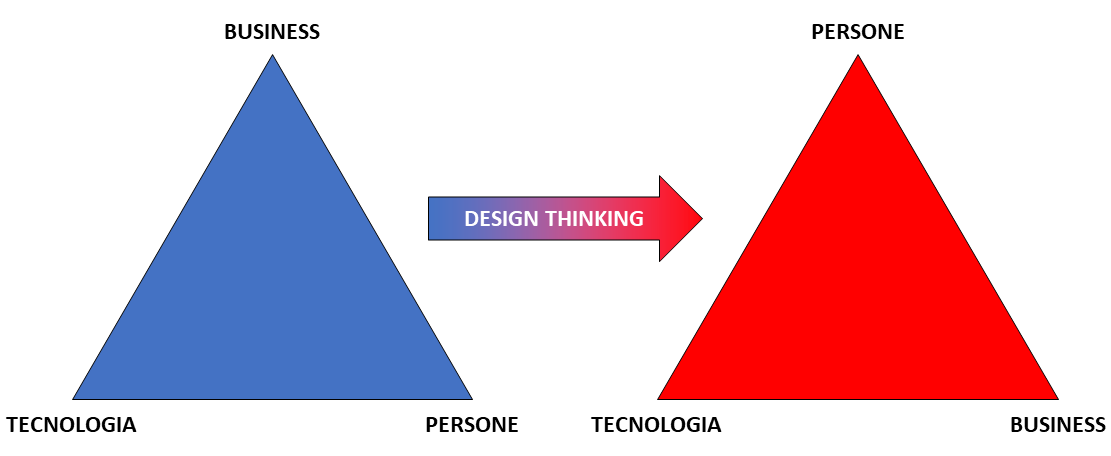
\includegraphics[width=\textwidth]{immagini/des_think.png}
	\caption{Nel design thinking gli obbiettivi della progettazione cambiano radicalmente. L'elemento di riferimento diventa l'utente e la sua soddisfazione, il business e la tecnologia sono solo degli strumenti per raggiungere questo obbiettivo.}
	\label{fig:dt_piramide}
\end{figure}

Questo diverso approccio assegna al termine design un significato nuovo, evidenziato del teorico del design Klaus Krippendorf che riporta il termine all’etimologia latina “de-signare”, e cioè, far sì che qualcosa si distingua attraverso un segno, dandogli un significato. 

Il processo di sviluppo mediante Design Thinking può essere suddiviso in 5 fasi principali:

\begin{itemize}
	\item \textbf{Empathize}: La prima fase consiste nell’identificazione del problema e quindi dell’obiettivo; 
	\item \textbf{Define}: La seconda fase è orientata a delineare meglio le domande chiave, cioè quali sono i bisogni degli utenti e quindi quali sono le varie categorie di utenti
	\item \textbf{Ideate}: La terza fase è quella orientata alla ricerca della soluzione, dell'opportunità tecnologica. In questa fase si fa uso di tecniche di stimolazione della creatività come brainstorming etc.;
	\item \textbf{Prototype}: La quarta fase è orientata alla realizzazione dei primi prototipi. Questa fase è molto importante per garantire un processo antropocentrico consentendo di andare il più velocemente possibile a testare il prodotto sul campo con gli utenti reali;
	\item \textbf{Test}: In fine la quinta fase è quella dedicata al test sul campo dei prototipi e alla raccolta dei feedback dagli utenti. Questa fase apparentemente conclusiva in realtà produce come output una serie di input per i futuri cicli di iterazione che si vanno ad applicare a tutte le fasi precedenti.
	
\end{itemize}

\begin{figure}
	\centering
	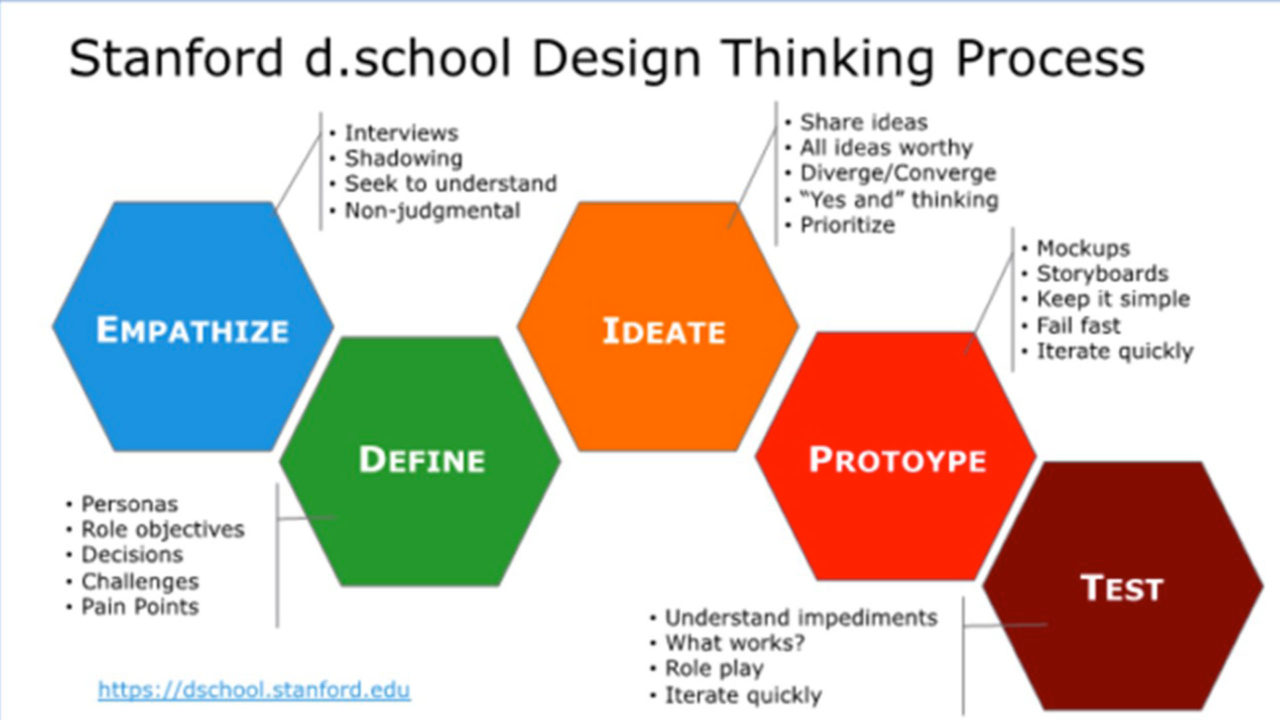
\includegraphics[width=\textwidth]{immagini/designthinking}
	\caption{Le 5 fasi del metodo Design Thinking. Fonte: https://www.zerounoweb.it/cio-innovation/metodologie/design-thinking-definizione-esempi/}
\end{figure}


Lo Human Centered Design è quindi un \textbf{mindset}, un modo di pensare e di approcciarsi allo sviluppo di prodotti. Come nel caso dello HCD Process, il Design Thinking, è invece un vero e proprio metodo di lavoro organizzato per fasi che consente di sviluppare prodotti centrati sull'utente grazie a tecniche orientate alla stimolazione della creatività e alla produzione di idee. Pensare di avviare un processo di disruptive innovation senza curarsi di progettare in maniera antropocentrica e senza un metodo di progettazione strutturato è al giorno d'oggi impossibile.

\begin{figure}
	\centering
	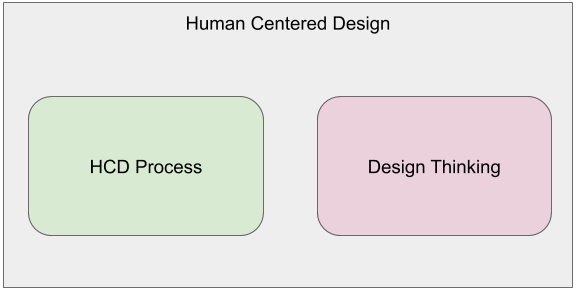
\includegraphics[width=0.6\textwidth]{immagini/dtvshcdp}
	\caption{HCD è una forma di pensiero, un approccio alla progettazione. HCD Process e Design Thinking sono invece metodi di progettazione molto utilizzati per il design di prodotti “disruptive”
}
\end{figure}

\section{Agile, Scrum e DevOps}
Nel mondo dello sviluppo software e dell'informatica in generale, negli utili anni si sono sviluppati molti metodi di organizzazione del lavoro orientati allo sviluppo veloce di sistemi innovativi. Tanti di questi metodi si basano su un mix di teorie e approcci di design applicati in altri settori e in generale puntano a dare al team di sviluppo un metodo di lavoro più snello, veloce e sopratutto orientato al prodotto e all'utente (antropocentrico).


Il metodo di sviluppo software classico, presentato come fondamento dell'ingegneria del software è sicuramente il modello Waterfall. In ingegneria del software, il modello a cascata (waterfall model in inglese) o ciclo di vita a cascata (waterfall lifecycle) è il più tradizionale modello di ciclo di vita del software. Secondo questo modello, il processo di realizzazione del software è strutturato in una sequenza lineare di fasi o passi, che comprende:

\begin{itemize}
    \item analisi dei requisiti
    \item progettazione
    \item sviluppo
    \item collaudo
    \item manutenzione

\end{itemize}

Questo modello riprende la sequenza di passi tipica della produzione manifatturiera, e fu il primo a essere applicato all'informatica quando lo sviluppo del software cominciò a essere concepito come attività industriale. Questo modello è stato progressivamente abbandonato dall'industria del software, ma rimane un importante riferimento storico.

Uno dei nuovi modelli di organizzazione dello sviluppo software che negli ultimi anni sta riscuotendo maggior successo è sicuramente l’Agile. Il metodo Agile nasce nel 2001 da un gruppo di 17 sviluppatori, che sentirono il bisogno di ripensare il loro modo di lavorare perchè stufi del classico metodo di sviluppo Waterfall. 
L'obbiettivo di questi sviluppatori era quello di progettare un nuovo metodo di lavoro orientato allo sviluppo di applicazioni software in maniera più leggera, economica e rapida. 




\begin{figure}[h!]
	\centering
	\includegraphics[width=\textwidth]{"immagini/agile_manifesto"}
\end{figure}

Produssero quindi un manifesto a partire dal quale sono stati sviluppati i 12 principi fondamentali dell'Agile:

\begin{enumerate}
    \item Our highest priority is to satisfy the customer
through early and continuous delivery
of valuable software.

\item Welcome changing requirements, even late in
development. Agile processes harness change for
the customer's competitive advantage.

\item Deliver working software frequently, from a
couple of weeks to a couple of months, with a
preference to the shorter timescale.

\item Business people and developers must work
together daily throughout the project.

\item Build projects around motivated individuals.
Give them the environment and support they need,
and trust them to get the job done.

\item The most efficient and effective method of
conveying information to and within a development
team is face-to-face conversation.

\item Working software is the primary measure of progress.

\item Agile processes promote sustainable development.
The sponsors, developers, and users should be able
to maintain a constant pace indefinitely.

\item Continuous attention to technical excellence
and good design enhances agility.

\item Simplicity--the art of maximizing the amount
of work not done--is essential.

\item The best architectures, requirements, and designs
emerge from self-organizing teams.

\item At regular intervals, the team reflects on how
to become more effective, then tunes and adjusts
its behavior accordingly.

\end{enumerate}


I principi riportati nel manifesto focalizzano lo sviluppo del software sugli individui e le interazioni, sul prodotto realizzato piuttosto che sulla documentazione, sull’interazione stretta con il cliente (utente) e soprattutto sui cambiamenti che possono avvenire anche durante lo sviluppo stesso del prodotto o servizio.

In sostanza, nello sviluppo Agile, si procede con un team molto coeso, composto da product manager e sviluppatori, a definire i requirement per uno sviluppo di una prima parte dell’applicazione, fermandosi poi a provare quanto realizzato, a ragionarci su e definire nuovi requirement per la realizzazione di nuove funzioni o di una revisione di quanto realizzato.

Questa metodologia di sviluppo veloce e libero ha avuto una spinta notevole dall’avvento della tecnologia Cloud, che ha favorito il deploy continuo del software consentendo quindi di velocizzare i cicli di sviluppo e test delle applicazioni.
Dalla Agile sono nate poi varie sotto-tecniche e metodi di organizzazione dello sviluppo software di cui lo \textbf{Scrum} è sicuramente una delle più diffuse. 

Scrum si basa sulla teoria dei controlli empirici di analisi strumentale e funzionale di processo o empirismo. L'empirismo afferma che la conoscenza deriva dall'esperienza e che le decisioni si basano su ciò che si conosce. Scrum utilizza un metodo interattivo ed un approccio incrementale per ottimizzare la prevedibilità ed il controllo del rischio.
In maniera molto sintetica, Scrum è un framework di processo che prevede di dividere il progetto in blocchi rapidi di lavoro \textbf{(Sprint)} alla fine di ciascuno dei quali creare un incremento del software. Esso indica come definire i dettagli del lavoro da fare nell'immediato futuro e prevede vari meeting con caratteristiche precise per creare occasioni di ispezione e controllo del lavoro svolto.

Il framework Scrum è profondamente antropocentrico. Ogni parte del framework serve a uno specifico scopo ed è essenziale per il successo e l'utilizzo di Scrum. Le regole di Scrum legano insieme gli eventi, i ruoli e gli artefatti governando le relazioni e le interazioni tra essi anche se le strategie specifiche per l'utilizzo del framework Scrum variano e vengono descritte in molti testi specifici.

Le persone che ricoprono i ruoli principali nel processo Scrum costituiscono il Team Scrum e sono quelle impegnate nel progetto e che realizzano il prodotto (obiettivo del progetto). Il Team Scrum è formato dal Product Owner, Il Team di sviluppo (Development Team) e da uno Scrum Master. \textbf{Il Product Owner rappresenta gli stakeholders ed è la voce del cliente.} È responsabile per assicurare che il team fornisca valore al business. Il Product Owner definisce gli item (requisiti di prodotto) centrati sui bisogni dei clienti (HCD), assegna loro la priorità, e li aggiunge al product backlog. I team Scrum debbono avere un Product Owner e si raccomanda che questo ruolo non sia combinato con quello dello ScrumMaster.

\begin{figure}[h!]
	\centering
	
		\includegraphics[width=\textwidth]{"immagini/Scrum-Agile-Marketing"}
		%\includegraphics[width=\textwidth]{"immagini/agile"}
	\caption{Nella metodologia Agile Scrum si lavora in cicli (sprint) composti da fasi successive in cui si sviluppa, si testa e si modifica sulla base del risultato dei test il codice sviluppato.}
\end{figure}

L'integrazione dei metodi Agile con il mondo del cloud, dei micro servizi e della programmazione server-less ha portato negli ultimi anni (2009) alla nascita di un nuovo metodo di sviluppo DevOps.

Il DevOps prevede, attraverso la collaborazione e integrazione tra sviluppatori e addetti alle operation la gestione più flessibile, affidabile, sicura e controllabile dei rilasci, tale da rendere più veloci i cicli di sviluppo e rilascio. Il DevOps si ispira alla metodologia Agile, alla necessità di incrementare la frequenza dei rilasci in produzione e fa leva sulla disponibilità di infrastrutture virtualizzate e in cloud.

\begin{figure}[h!]
	\centering
	\includegraphics[width=0.7\textwidth]{"immagini/devops-process"}
	\caption{Ciclo DevOps. Fonte https://italiancoders.it/introduzione-al-devops/.}
\end{figure}

\section{Analisi delle Cause Profonde}
\textit{ \tiny Tratto da: https://www.tableau.com/it-it/learn/articles/root-cause-analysis}\\


La Agile e la Scrum abbiamo detto essere delle tecniche basate su cicli di sviluppo e verifica basati su un forte impianto empiristico. queste tecniche prevedono quindi che una volta sviluppato del software si eseguano dei test, si analizzino i problemi e si lavori per risolvere le cause che hanno generato i malfunzionamenti identificati o hanno comportato frustrazione nel cliente/utente.

L'identificazione delle cause di un problema sembra un processo banale ma in realtà è un'attività estremamente complessa. Spesso infatti, si tende a confondere il problema con il sintomo che questo comporta. e' tipicamente semplice eliminare il sintomo ma è spesso molto complesso eliminare la causa.

\textit{Se avete la tosse, prenderete una caramella al miele vi passerà la tosse (il sintomo) per qualche minuto ma poi la tosse tornerà perchè la causa scatenante non è stata rimossa e quindi il problema è ancora presente e il sintomo si ripresenterà.}

L'analisi delle cause profonde (RCA, Root cause analysis) è un procedimento finalizzato all'identificazione delle cause poste alla radice di un problema. L'obbiettivo della RCA è quindi quello di risolvere i problemi all'origine andando oltre la semplice tacitazione dei sintomi. L'RCA parte dal presupposto che sia molto più utile prevenire e risolvere le problematiche sottostanti in modo sistematico invece di trattare semplicemente i sintomi e arginare il problema caso per caso.

La RCA è quindi uno strumento fondamentale per la gestione dei processi di sviluppo di tipo Agile.

L'analisi delle cause profonde può essere eseguita con l'aiuto di vari principi, tecniche e metodologie da mettere in pratica per identificare le cause alla radice di un evento o di un trend. L'RCA scava più a fondo della causa e dell'effetto in superficie ed è in grado di evidenziare le lacune dei processi e dei sistemi o il motivo alla base dell'insorgenza di un problema.

Obiettivi e vantaggi della RCA:
\begin{enumerate}
    \item Il primo obiettivo dell'analisi delle cause profonde è scoprire la causa all'origine di un problema o di un evento.
    \item Il secondo obiettivo è comprendere appieno come correggere e trovare un rimedio alle problematiche sottostanti all'interno della causa principale, oltre a imparare da queste.
    \item Il terzo obiettivo è applicare quanto imparato da questa analisi per impedire in modo sistematico problematiche future o per ottenere di nuovo risultati positivi.

\end{enumerate}

Ciò che facciamo con i risultati di questa analisi è importante quanto l'analisi stessa e quindi il terzo obiettivo ha una rilevanza da non sottovalutare. Possiamo utilizzare l'RCA anche per modificare le problematiche principali dei processi e dei sistemi in modo da evitare che si verifichino problemi in futuro. Invece di trattare semplicemente i sintomi di una commozione cerebrale di un rugbista, ad esempio, l'analisi delle cause profonde può suggerire di fargli indossare un caschetto per ridurre il rischio di traumi futuri.

Trattare i sintomi uno per uno può sembrare produttivo e risolvere un ampio numero di problemi dà l'impressione di aver trovato una soluzione efficace (tipico dei processi di debug del software). Tuttavia, se ignoriamo la diagnosi effettiva della vera causa scatenante, lo stesso identico problema potrebbe ripresentarsi ancora e ancora. 

Invece di incaricare un redattore di correggere ogni singola virgola omessa, insegnare agli scrittori a usare correttamente la punteggiatura permetterebbe di non affrontare più queste problematiche in testi futuri.

Alla base di un'efficace analisi delle cause profonde vi sono alcuni principi chiave, che in parte dovrebbero già essere evidenti. Questi non solo contribuiscono alla qualità dell'analisi, ma aiutano anche gli analisti a creare fiducia e ottenere l'approvazione di parti interessate, clienti o pazienti.

\begin{itemize}
    \item Punta a risolvere e trovare una soluzione per le cause profonde, non per i soli sintomi.
    \item Non ignorare l'importanza di trattare i sintomi per una soluzione a breve termine.
    \item Considera il fatto che possono esserci, e spesso ci sono, più cause profonde.
    \item Concentrati sul COME e sul PERCHÉ si è verificato un evento, non sul CHI ne è responsabile.
    \item Adotta un approccio metodico e trova le prove concrete della relazione di causa-effetto per avere una conferma delle cause profonde rilevate.
    \item Fornisci informazioni sufficienti per dare forma a un percorso di azioni correttivo.
    \item Valuta come evitare l'insorgenza (o il ripetersi) di una causa profonda in futuro.

\end{itemize}

Come risulta chiaro da questi principi, quando analizziamo le problematiche e le cause profonde, è importante adottare un approccio onnicomprensivo e olistico. Oltre a scoprire la causa profonda, dobbiamo fare in modo di raccogliere dati contestuali e informazioni sufficienti per intraprendere un'azione correttiva o prendere una decisione; \textbf{una buona analisi è un'analisi attuabile.}

Le tecniche e le strategie per l'analisi delle cause profonde sono numerosissime, il metodo dei 5 perchè è uno dei più utilizzati e semplici da capire.

\subsection{Metodo dei 5 Perché}
Una delle tecniche più seguite per effettuare un'analisi delle cause profonde è il metodo dei 5 Perché. È più o meno quello che succede quando i bambini chiedono tutti quei fastidiosi perché uno dietro all'altro, dove a ogni domanda ne segue un'altra concatenata e che scava sempre più a fondo. I bambini sono sorprendentemente bravi con l'analisi delle cause profonde. L'opinione diffusa è che siano sufficienti circa cinque PERCHÉ per identificare le principali cause profonde, ma potrebbero volercene un po' di meno o molti di più.

\textbf{Esempio:} prendiamo di nuovo l'esempio della commozione cerebrale del rugbista. \\

Prima di tutto, il giocatore solleva un problema: perché ho questo terribile mal di testa? Questo è il nostro primo PERCHÉ.
Prima risposta: perché ci vedo doppio.\\

Secondo perché: perché ci vedi doppio?
Seconda risposta: perché ho sbattuto la testa a terra.\\

Terzo perché: perché hai sbattuto la testa a terra?
Terza risposta: sono stato placcato e ho sbattuto la testa a terra.\\

Quarto perché: perché cadere a terra ti ha fatto così male?
Quarta risposta: perché non indossavo il caschetto.\\

Quinto perché: perché non indossavi un caschetto?
Quinta risposta: perché non c'erano abbastanza caschetti nello spogliatoio.

Ecco, dopo queste cinque domande abbiamo scoperto che la causa alla radice della commozione cerebrale è molto probabilmente una mancanza di caschetti disponibili. Per il futuro, possiamo ridurre il rischio di traumi di questo genere assicurandoci che ogni giocatore abbia un caschetto.

\textbf{Il metodo dei 5 Perché ci permette di non fare supposizioni}. Man mano che aumentano le domande, le risposte dettagliate diventano sempre più chiare e concise. In teoria, l'ultimo PERCHÉ porta a identificare una lacuna nel processo, che quindi può essere corretta.
